\documentclass[twocolumn]{article}

\usepackage{imr}
\usepackage{graphicx}
\usepackage{amsfonts}
\usepackage{bbm}       % for \mathbbm{1}
\usepackage{amsmath}
\usepackage{mathrsfs}  % for \mathscr
\usepackage{minted}    % for including source code
\usepackage{tikz}
\usetikzlibrary{decorations.markings}

\def\thepage {}
\bibliographystyle{imr}

\newenvironment{smallarray}[1]
 {\null\,\vcenter\bgroup\scriptsize
  \renewcommand{\arraystretch}{0.7}%
  \arraycolsep=.13885em
  \hbox\bgroup$\array{@{}#1@{}}}
 {\endarray$\egroup\egroup\,\null}

\begin{document}

\title{An ergonomic approach to topological transformations of unstructured meshes}
\author{Daniel Shapero$^1$}
\date{
    $^1$University of Washington, Seattle, WA, USA, shapero@uw.edu
}

\abstract{In this paper, we will describe an approach to performing local transformations to the topology of an unstructured mesh.
Our approach borrows some ideas from algebraic topology and makes for much easier verification of the underlying computational kernels.}

\keywords{mesh generation, computational geometry, topology}

\maketitle
\thispagestyle{empty}
\pagestyle{empty}


% --------------------
\section{Introduction}

All algorithms for generating unstructured meshes are based on applying a sequence of local transformations to the mesh topology.
For example, to compute the Delaunay triangulation, the Lawson algorithm uses a sequence of bistellar flips, while the Bowyer-Watson algorithm is based on splitting star-shaped polytopes along a vertex \cite{berg1997computational, cheng2013delaunay}.
Implementing these transformations, however, can be difficult and error-prone.

In this paper, we will describe a method for implementing local topological transformations using concepts from algebraic topology: the \emph{boundary operators} of a \emph{chain complex}.
These boundary operators are really just matrices with integer coefficients.
We can then describe transformations using linear algebra.
This idea is not new; DiCarlo and others \cite{dicarlo2007solid} used chain complexes to implement the Euler make/kill operators from solid modeling.
Our contribution is a linear algebraic representation of splitting a star-shaped collection of polygons on a new vertex.
The key result is in equations \eqref{eq:split-k} and \eqref{eq:split-n}.


% -----------------------
\section{Chain complexes}

Here we briefly recall some definitions; see \cite{hatcher2002algebraic} for all the formalities.
A 0-dimensional cell complex $X^0$ is a finite collection of points.
A regular $n$-dimensional cell complex consists of an $n - 1$-dimensional cell complex $X^{n - 1}$ together with a collection $\{\phi_\alpha^n\}$ of homeomorphisms, called \emph{attaching maps}, from the unit sphere in $S^{n - 1}$ into $X^{n - 1}$.
The space $X^n$ is then the disjoint union of copies of the unit ball with each copy's boundary identified with its image in $X^{n - 1}$ under the attaching map with the quotient topology.
Both simplicial and cubical complexes are cell complexes.

Given a $k$-cell $\sigma$ and a $k - 1$-cell $\tau$ of a complex $X$, we can define the \emph{incidence number} as
\begin{equation}
    [\sigma, \tau] = \begin{cases}0 & \tau\text{ is not in }\sigma \\ +1 & \tau \text{ is positively oriented in }\sigma \\ -1 & \tau\text{ is negatively oriented in }\sigma\end{cases}
\end{equation}
The formal definition of incidence number uses the topological degree of the attaching map $\phi$ of $\tau$ into $\partial\sigma$, which we will not define here.
For simplicial and cubical complexes, the incidence numbers between cells can be read off directly from their constituent vertexes.

The key object of interest for us is the \emph{boundary operator} on a cell complex.
The \emph{chain module} $\mathscr{C}_k$ is the set of all formal $\mathbb{Z}$-linear combinations of cells of dimension $k$.
Given a single $k$-cell $\sigma$ of $X$, we define
\begin{equation}
    \partial_k\sigma = \sum_{\tau \in X^{k - 1}}[\sigma, \tau]\tau
\end{equation}
and extend $\partial_k$ by $\mathbb{Z}$-linearity to a map from $\mathscr{C}_k$ to $\mathscr{C}_{k - 1}$.
The most important fact about boundary operators and the wellspring of homology theory is that
\begin{equation}
    \partial_k\cdot\partial_{k + 1} = 0.
    \label{eq:ddzero}
\end{equation}
A collection of $\mathbb{Z}$-modules $\mathscr{C}_k$ together with homomorphisms $\partial_k : \mathscr{C}_k \to \mathscr{C}_{k - 1}$ that satisfy equation \eqref{eq:ddzero} is called a \emph{chain complex}.

% TODO: Add labels to the figure and the boundary matrices, see
% https://tex.stackexchange.com/a/59732
\begin{figure}[h]
    \begin{minipage}{0.48\linewidth}
        \begin{center}
            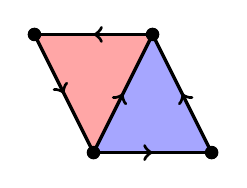
\begin{tikzpicture}[scale=0.75]
                \coordinate (p1) at (1, 0){};
                \coordinate (p2) at (3, 0){};
                \coordinate (p3) at (2, 2){};
                \coordinate (p4) at (0, 2){};

                \draw[fill=blue!35] (p1) -- (p2) -- (p3) -- cycle;
                \draw[fill=red!35] (p1) -- (p3) -- (p4) -- cycle;
                \begin{scope}[
                    very thick,
                    decoration={markings, mark=at position 0.5 with {\arrow{>}}}
                ]
                    \draw[postaction={decorate}] (p1) -- (p2);
                    \draw[postaction={decorate}] (p2) -- (p3);
                    \draw[postaction={decorate}] (p3) -- (p4);
                    \draw[postaction={decorate}] (p4) -- (p1);
                    \draw[postaction={decorate}] (p1) -- (p3);
                \end{scope}
                \foreach \p in {p1, p2, p3, p4} {
                    \filldraw (\p) circle (3pt);
                }
            \end{tikzpicture}
        \end{center}
    \end{minipage}
    \hfill
    \begin{minipage}{0.48\linewidth}
        {\small
            \begin{equation*}
                \partial_1 = \left[\begin{smallmatrix}
                    - &   & + & - &   \\
                    + & - &   &   & + \\
                      & + & - &   &   \\
                      &   &   & + & -
                \end{smallmatrix}\right]
            \end{equation*}
            \begin{equation*}
                \partial_2 = \left[\begin{smallmatrix}
                    + & - \\
                    + &   \\
                    + &   \\
                      & + \\
                      & +
                \end{smallmatrix}\right]
            \end{equation*}
        }
    \end{minipage}
    \caption{Pair of adjacent triangles (left) and their boundary matrices (right).}
    \label{fig:two-triangle-chain-complex}
\end{figure}

The abstract concept of a cell complex can be made computable by representing its boundary operators as (sparse) matrices with integer entries.
We can read off the faces and sub-faces of a particular cell by looking at which rows are non-zero in the corresponding columns of the boundary matrices.
See figure \ref{fig:two-triangle-chain-complex} for an illustration of a simple topology together with the corresponding boundary operators.

We'll introduce one final conceit that makes later constructions much more elegant.
The definition above assumes that the chain complex stops at $\mathscr{C}_0$ -- formal linear combinations of vertices.
Instead, we will add a \emph{bottom} module $\mathscr{C}_{-1}$ consisting of a single cell $\bot$ of dimension -1.
We then define the boundary of every vertex $v_i$ to be $+\bot$.
If we write $\mathbbm{1}$ for the column vector of all 1s, then $\partial_0 = \mathbbm{1}^*$, i.e. the row vector of all 1s.
The addition of this bottom cell is especially convenient because the condition $\partial_0\partial_1 = 0$ implies that the boundary of every edge $e$ has a negative and a positive vertex: $\partial e = v_i - v_j$ for some $i$, $j$.
We cannot have, for example, $\partial e = v_i + v_j$, which would be undesirable.


% -----------------------
\section{Transformations}

If we choose to represent mesh topologies using boundary operators, we can describe transformations through linear algebra.
Phrasing the problem in this way makes verifying correctness easy.

First, observe that if $A$, $B$ are integer matrices such that the image of $\partial_{k + 1}$ is an invariant subspace of $A\cdot B$, then the matrices
\begin{equation}
    \partial_k' = \partial_k\cdot A, \quad \partial_{k + 1}' = B\cdot\partial_{k + 1}
\end{equation}
still satisfy $\partial_k'\cdot\partial_{k + 1}' = 0$.
A particular case is $A\cdot B = I$, which includes permutations of the cell ordering.
The more general case regarding the image of $A\cdot B$ is needed for some irreversible transformations.

\subsection{Merging}

A \emph{merge} of a set of $k$-cells replaces them with a single cell (provided that their union is simply-connected).
Merging is a column operation on the matrix $\partial_k$.
In the simplest case, the result column is the sum of all the columns to be merged, but in general we might need to flip some signs:
\begin{align}
    \partial_k' & = \partial_k\cdot\text{diag}(s_0, \ldots, s_m)\cdot\mathbbm{1}, \\
    \partial_{k + 1}' & = \left[\begin{matrix} 0 \ldots 1 \ldots 0\end{matrix}\right]\partial_{k + 1}. \label{eq:merge-k+1}
\end{align}
where $s_i$ are all $\pm 1$.
The signs are chosen so that any higher-dimensional cell $\sigma$ has the same incidence with respect to any of the cells $\tau$ to be merged.
The transformation to the rows of $\partial_{k + 1}$ collapses all incidence to any of the desired $k$-cells into incidence to the merged $k$-cell.
For merging cells of top dimension $n$, there are no higher-dimensional cells to apply equation \eqref{eq:merge-k+1} to and this step is left out.

\emph{Edge collapsing}, the key transformation in surface simplification algorithms \cite{gueziec1995surface}, is a merge of two vertices.


\subsection{Splitting}

A \emph{split} divides up the union of several polytopes along a point.
The key correctness criteria for this operation are that (1) every newly-created polytope contains the splitting point and (2) the boundary of the sum of all polytopes does not change.
We'll first describe the 2D case and then proceed to arbitrary dimensions.

Suppose that a collection of adjacent polygons has the boundary operators $\partial_1$ and $\partial_2$.
We first have to draw edges between the new vertex and all the vertices of the polygon.
The orientation of these new edges is arbitrary, so we can assume that every edge goes from the splitting vertex $v$ to the polygon vertices.
Another way of stating this is that every new edge $e$ is negatively-incident to $v$ and positively-incident to some polygon vertex.
In terms of matrices, the new 1-boundary operator is
\begin{equation}
    \partial_1' = \left[\begin{matrix}\partial_1 & I \\ 0 & -\mathbbm{1}^*\end{matrix}\right]
    \label{eq:split-1-2d}
\end{equation}
where $I$ is the identity matrix.
The key step here is defining the 2-boundary matrix:
\begin{equation}
    \partial_2' = \left[\begin{matrix}\text{diag}(\partial_2\cdot\mathbbm{1}) \\ -\partial_1\cdot\text{diag}(\partial_2\cdot\mathbbm{1})\end{matrix}\right]
\end{equation}
A rudimentary calculation shows that $\partial_1'\partial_2' = 0$.
Since $\text{diag}(z)\cdot\mathbbm{1} = z$ for any vector $z$, we also find that
\begin{equation}
    \partial_2'\mathbbm{1} = \left[\begin{matrix}\partial_2\mathbbm{1} \\ 0\end{matrix}\right]
\end{equation}
or in other words the new polygon has the same boundary as the old.
Figure \ref{fig:split-transformation} illustrates the split transformation on a single quadrilateral and shows the boundary matrices before and after.

\begin{figure}[h]
    \begin{center}
        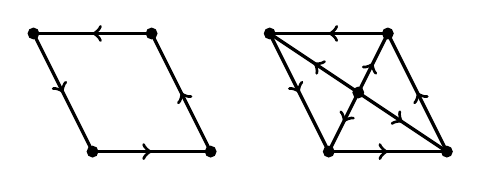
\begin{tikzpicture}[scale=0.75]
            \newcommand*{\defcoords}{
                \coordinate (p0) at (1.5, 1){};
                \coordinate (p1) at (1, 0){};
                \coordinate (p2) at (3, 0){};
                \coordinate (p3) at (2, 2){};
                \coordinate (p4) at (0, 2){};
            }

            \begin{scope}[
                very thick,
                decoration={markings, mark=at position 0.5 with {\arrow{>}}}
            ]
                \defcoords
                \draw[postaction={decorate}] (p1) -- (p2);
                \draw[postaction={decorate}] (p2) -- (p3);
                \draw[postaction={decorate}] (p3) -- (p4);
                \draw[postaction={decorate}] (p4) -- (p1);

                \foreach \p in {p1, p2, p3, p4} {
                    \filldraw (\p) circle (2pt);
                }
            \end{scope}

            \begin{scope}[
                very thick,
                shift={(4, 0)},
                decoration={markings, mark=at position 0.5 with {\arrow{>}}}
            ]
                \defcoords
                \draw[postaction={decorate}] (p1) -- (p2);
                \draw[postaction={decorate}] (p2) -- (p3);
                \draw[postaction={decorate}] (p3) -- (p4);
                \draw[postaction={decorate}] (p4) -- (p1);
                \draw[postaction={decorate}] (p0) -- (p2);
                \draw[postaction={decorate}] (p0) -- (p3);
                \draw[postaction={decorate}] (p0) -- (p4);
                \draw[postaction={decorate}] (p0) -- (p1);

                \foreach \p in {p0, p1, p2, p3, p4} {
                    \filldraw (\p) circle (2pt);
                }
            \end{scope}
        \end{tikzpicture}
    \end{center}

    \begin{equation*}
        \partial_1 = \left[\begin{smallmatrix}
            - &   &   & + \\
            + & - &   &   \\
              & + & - &   \\
              &   & + & -
        \end{smallmatrix}\right],
        \quad
        \partial_2 = \left[\begin{smallmatrix}
            + \\ + \\ + \\ +
        \end{smallmatrix}\right]
    \end{equation*}

    \begin{equation*}
        \partial_1' = \left[\begin{smallarray}{cccc|cccc}
            - &   &   & + & + &   &   &   \\
            + & - &   &   &   & + &   &   \\
              & + & - &   &   &   & + &   \\
              &   & + & - &   &   &   & + \\
            \hline
              &   &   &   & - & - & - & -
        \end{smallarray}\right], \quad
        \partial_2' = \left[\begin{smallarray}{cccc}
            + &   &   &   \\
              & + &   &   \\
              &   & + &   \\
              &   &   & + \\
            \hline
            + &   &   & - \\
            - & + &   &   \\
              & - & + &   \\
              &   & - & +
        \end{smallarray}\right]
    \end{equation*}

    \caption{Quadrilateral before and after splitting on a new vertex in the center (top) and boundary matrices before and after (bottom).}
    \label{fig:split-transformation}
\end{figure}

We can get an idea for how to extend this to $n$ dimensions by remembering that $\mathbbm{1}^* = \partial_0$ in equation \eqref{eq:split-1-2d}.
This suggests the transformation
\begin{align}
    \partial_k' & = \left[\begin{matrix}\partial_k & I \\ 0 & -\partial_{k - 1}\end{matrix}\right] \label{eq:split-k} \\
    \partial_n' & = \left[\begin{matrix}\text{diag}(\partial_n\cdot\mathbbm{1}) \\ -\partial_{n - 1}\text{diag}(\partial_n\cdot\mathbbm{1})\end{matrix}\right] \label{eq:split-n}
\end{align}
Again, a rudimentary calculation shows that the fundamental equation \eqref{eq:ddzero} still holds and that the new polytopes have the same boundary as the old.

Equation \eqref{eq:split-k} has appeared before in the literature on homological algebra as the expression for the boundary operators of the \emph{cone} of a space \cite{gelfand1994homological}.
To our knowledge, using these equations for doing real computations is entirely new.

The Bowyer-Watson algorithm for Delaunay triangulation and all common algorithms for computing convex hulls only require the split transformation \cite{berg1997computational}.

\subsection{Splitting and merging}

Other transformations can be defined by combining a sequence of splits and merges.
For example, figure \ref{fig:2-2-flip} shows how to perform a 2-2 flip in 2D by first splitting the quadrilateral into four triangles and then performing a sequence of merges and figure \ref{fig:2-3-flip} shows the same process for a 2-3 flip in 3D.
(We've shown an initial merge step for illustrative purposes, but this merge is actually part of the subsequent split.)

\begin{figure}[h]
    \tikzset{ec/.style={every coordinate/.try}}

    \begin{center}
    \begin{tikzpicture}[scale=0.4]
        \coordinate (p0) at (1.5, 1){};
        \coordinate (p1) at (1, 0){};
        \coordinate (p2) at (3, 0){};
        \coordinate (p3) at (2, 2){};
        \coordinate (p4) at (0, 2){};

        \begin{scope}[very thick]
            \draw (p1) -- (p2) -- (p4) -- cycle;
            \draw (p4) -- (p3) -- (p2) -- cycle;

            \foreach \p in {p1, p2, p3, p4} {
                \filldraw (\p) circle (3pt);
            }
        \end{scope}

        \begin{scope}[very thick, every coordinate/.style={shift={(3.5,0)}}]
            \draw ([ec]p1) -- ([ec]p2) -- ([ec]p3) -- ([ec]p4) -- cycle;

            \foreach \p in {p1, p2, p3, p4} {
                \filldraw ([ec]\p) circle (3pt);
            }
        \end{scope}

        \begin{scope}[very thick, every coordinate/.style={shift={(7,0)}}]
            \draw ([ec]p0) -- ([ec]p1) -- ([ec]p2) -- cycle;
            \draw ([ec]p0) -- ([ec]p2) -- ([ec]p3) -- cycle;
            \draw ([ec]p0) -- ([ec]p3) -- ([ec]p4) -- cycle;
            \draw ([ec]p0) -- ([ec]p4) -- ([ec]p1) -- cycle;

            \foreach \p in {p0, p1, p2, p3, p4} {
                \filldraw ([ec]\p) circle (3pt);
            }
        \end{scope}

        \begin{scope}[very thick, every coordinate/.style={shift={(10.5,0)}}]
            \draw ([ec]p1) -- ([ec]p2) -- ([ec]p3) -- cycle;
            \draw ([ec]p3) -- ([ec]p4) -- ([ec]p1) -- cycle;

            \foreach \p in {p0, p1, p2, p3, p4} {
                \filldraw ([ec]\p) circle (3pt);
            }
        \end{scope}

        \begin{scope}[very thick, every coordinate/.style={shift={(14,0)}}]
            \draw ([ec]p1) -- ([ec]p2) -- ([ec]p3) -- cycle;
            \draw ([ec]p3) -- ([ec]p4) -- ([ec]p1) -- cycle;

            \foreach \p in {p1, p2, p3, p4} {
                \filldraw ([ec]\p) circle (3pt);
            }
        \end{scope}

        \begin{scope}[very thick]
            \draw[->] (2, -0.2) arc[start angle=180, end angle=360, radius=1.5] node[midway, below, align=center] {merge\\triangles};
            \draw[->] (5.5, -0.2) arc[start angle=180, end angle=360, radius=1.5] node[midway, below] {split};
            \draw[->] (9.0, -0.2) arc[start angle=180, end angle=360, radius=1.5] node[midway, below, align=center] {merge\\triangles};
            \draw[->] (12.5, -0.2) arc[start angle=180, end angle=360, radius=1.5] node[midway, below, align=center] {merge\\edges};
        \end{scope}
    \end{tikzpicture}
    \end{center}
    \caption{A 2-2 flip, implemented as a sequence of merges and splits.
    The vertex added by splitting the quadrilateral is deleted when the two edges are merged in the final transformation.}
    \label{fig:2-2-flip}
\end{figure}

\begin{figure}[h]
    \begin{center}
        \input{figures/tetrahedra.tikz}
    \end{center}
    \caption{A 2-3 flip implemented as a sequence of merges and splits.
    We've shown the tetrahedra in an ``exploded'' view to help with visualization.}
    \label{fig:2-3-flip}
\end{figure}

A few papers have proposed using multi-cell transformations for 3D mesh improvement \cite{klingner2008aggressive}.
Multi-cell transformations are more complex than 2-3 or 3-2 flips, but \cite{misztal2009tetrahedral} showed that they can be implemented as a sequence of 2-3 and 3-2 flips.
Using the boundary operator representation might make it possible to implement complex topological transforms with less effort and in fewer steps.


% ---------------------
\section{Demonstration}

As a proof of concept, we developed a software package called \emph{zmsh}
which implements the split transformation defined in equations \eqref{eq:split-k} and \eqref{eq:split-n}.
The source code for the split transformation is shown in figure \ref{fig:split-source-code}.
\begin{figure}
    \begin{minted}[fontsize=\footnotesize,linenos]{python}
import numpy as np
from typing import List

def split(D: List[np.ndarray]) -> List[np.ndarray]:
    # Create the boundary matrices for 1 <= k < n
    n_vertices = D[0].shape[1]
    E = [np.ones((1, n_vertices + 1), int)]
    for k in range(1, len(D) - 1):
        n_cells = D[k].shape[1]
        n_sub_faces, n_faces = D[k - 1].shape
        I = np.identity(n_faces, int)
        Z = np.zeros((n_sub_faces, n_cells), int)
        E_k = np.block([[D[k], I], [Z, -D[k - 1]]])
        E.append(E_k)

    # Create the top-dimensional boundary matrix
    C = np.diag(np.sum(D[-1], axis=1))
    E_n = np.vstack((C, -D[-2] @ C))
    E.append(E_n)
    return E
    \end{minted}
    \caption{Python source code for the split transformation.
    Line 13 corresponds to equation \eqref{eq:split-k}; lines 17 and 18 correspond to equation \eqref{eq:split-n}.
    The real version has some additional logic to remove empty cells.}
    \label{fig:split-source-code}
\end{figure}
We used the split transformation to implement a convex hull algorithm that works in arbitrary dimensions.
To test the convex hull code, we used (1) random point sets up to dimension 5 and (2) several synthetic input sets with various degeneracies such as coplanarity.
For geometric predicates, we used the Python standard library's built-in routines to convert a floating point value exactly to a ratio of big integers.


% ------------------
\section{Conclusion}

Doubly-connected edge lists have historically been popular for mesh generation because they offer a simple interface for traversing the topology \cite{guibas1985primitives}.
Here we propose that boundary operators are an ideal representation if the goal is to perform topological transformations.
This idea has appeared before, for example in the work of DiCarlo and others \cite{dicarlo2007solid}.

Boundary operators are only necessary for representing a small patch of the topology at a time.
Once the transformed patch is computed, it can be translated back to a set of simplexes.
Boundary operators are useful for describing non-simplicial intermediate states of a transformation; they are not space-optimal for describing an entire simplicial complex.

When the underlying objects of study can be represented as linear operators, we can apply linear algebraic reasoning to define transformations and verify that they preserve all of the important invariants.
The condition in equation \eqref{eq:ddzero} that the product of two boundary operators is zero is a very powerful invariant for ensuring the validity of the underlying topology.


\bibliography{chain-complexes.bib}

\end{document}
